% !TEX encoding = UTF-8
% !TEX TS-program = pdflatex
% !TEX root = ../Tesi.tex
% !TEX spellcheck = it-IT

%************************************************
\chapter{Optimal reciprocal Collision Avoidance}
\label{cap:orca}
%************************************************

Optimal reciprocal Collision Avoidance \textit{ORCA} \'e un algoritmo basato su VO. 
Con questo procedimento si riduce il problema del \textit{collision-free} con una soluzione lineare computazionalmente ridotta. Ottimo anche per simulazioni popolate da centinaia di robot in uno spazio di lavoro limitato.

\section{Optimal reciprocal Collision Avoidance}

Come gli altri algoritmi precedentemente osservati, ogni robot tiene conto della velocit\'a, del raggio e della posizione corrente osservata dagli altri robot al fine di evitare collisioni. Inoltre pu\'o selezionare la sua velocit\'a dal suo spazio velocit\'a (\textit{velocity space}), dove alcune aree di questo spazio sono state etichettate come ''proibite'', per la presenza di altri robot. \\Questa formulazione, per ogni robot, crea un semipiano (\textit{half-plane}) delle velocit\'a dove è consentito essere per non avere delle collisioni. Perci\'o il robot selezioner\'a la nuova velocit\'a ottimale ({\bfseries\textit{v}\ap{opt}}) dalla intersezione di tutti i semipiani dove consentito essere. Per computare la nuova velocit\'a, si pu\'o utilizzare in modo efficente la programmazione lineare (\textit{linear programming}). In determinate condizioni, con densit\'a di robot elevate, la programmazione lineare potrebbe non trovare un risultato, in questo caso selezioniamo la pi\'u sicura velocit\'a possibile aggiungendo una terza dimensione alla programmazione lineare.

\subsection{Definition}
Dalle informazioni riportate precedentemente, selezioniamo per i robot \textit{A} e \textit{B} l'insieme delle velocit\'a permesse, che chiameremo {\bfseries\textit{V}\ped{A}} e {\bfseries\textit{V}\ped{B}}  tale che {\bfseries\textit{V}\ped{A}} sia equivalente al cono delle collisioni (${CC}_{A,B}\simeq CA^\tau_{A,B}(V_B)$) con un determinato \textit{time horizon}, {$\tau$}, che permette di creare un tronco di cono con apice nell'origine delimitato da due rette tangenti  a \textit{r}\ped a+\textit{r}\ped b, centrate in \textit{p}\ped{b} - \textit{p}\ped{a}. La dimensione della parte troncata dipende dal valore di $\tau$; il cono \'e troncato da un arco di raggio $\frac{r_a+r_b}{\tau}$ centrato in $\frac{p_b-p_a}{\tau}$. Equivalentemente per {\bfseries\textit{V}\ped{B}} tale che $CA^\tau_{B,A}(V_A)={V}_{B}$, queste aree garantiscono l'anticollisione per almeno un certo tempo $\tau$. 
\\Per ogni area viene creato un insieme di velocit\'a vicine alle velocit\'a ottimali (\textit{optimization velocities}) {\bfseries\textit{v}\ap{opt}\ped{A}} per \textit{A} e {\bfseries\textit{v}\ap{opt}\ped{B}} per \textit{B}, tale che noi denoteremo questi insiemi come \textit{ORCA}\ap{$\tau$}\ped{A,B} per \textit{A} e \textit{ORCA}\ap{$\tau$}\ped{B,A} per \textit{B}, definiti formalmente come segue:

\begin{figure}
\centering 
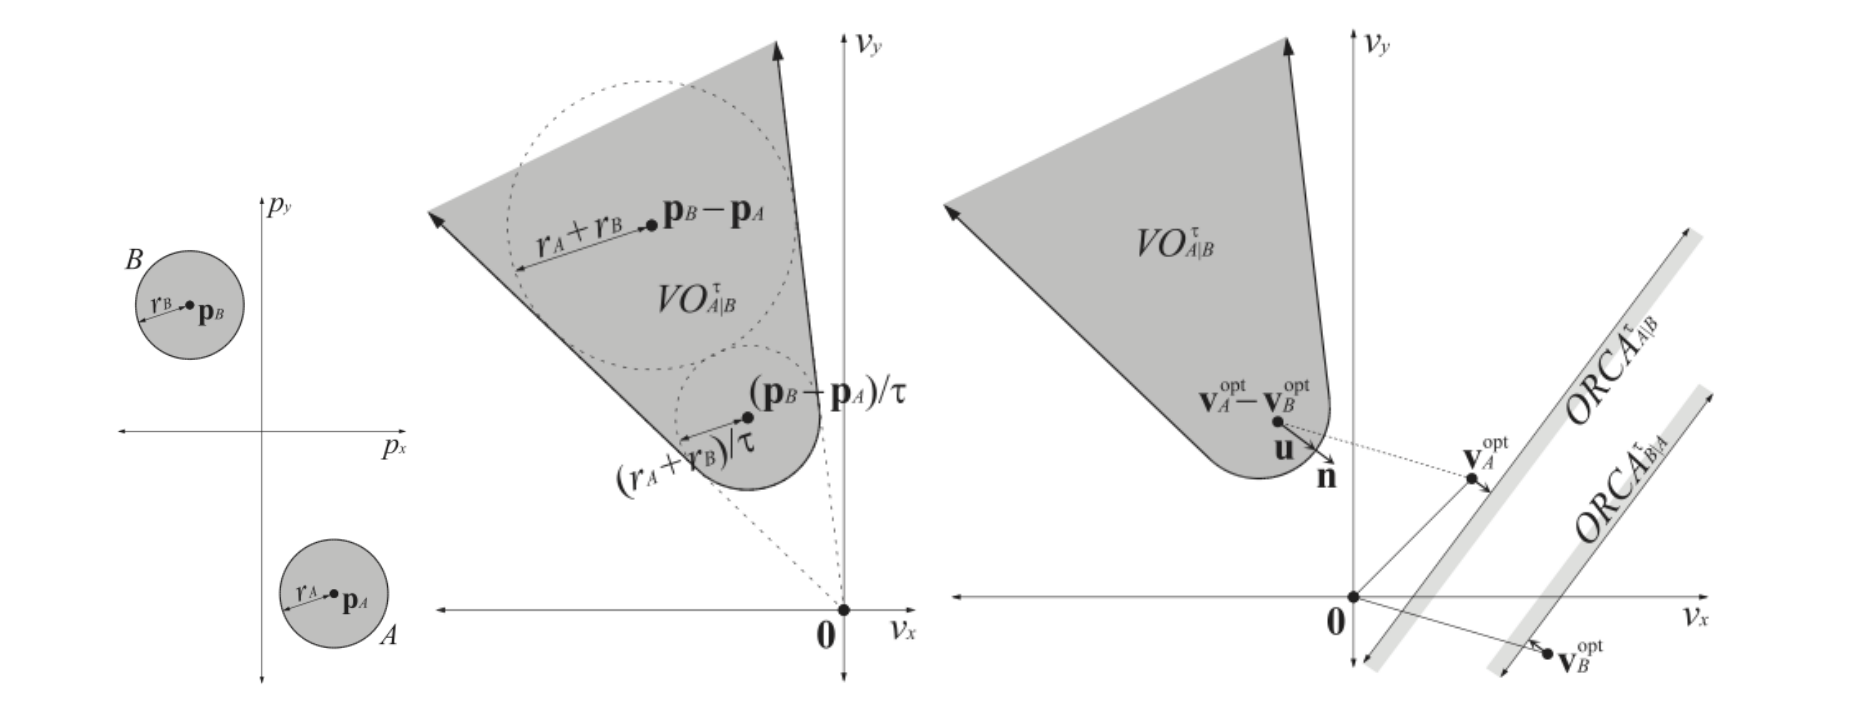
\includegraphics[width=0.8\columnwidth]{orca} 
\caption[Costruzione del cono VO\ped{A,B} con un determinato $\tau$ e la delimitazione del semipiano delle ORCA\ped{A,B} e ORCA\ped{B,A}]{Costruzione del cono VO\ped{A,B} con un determinato $\tau$ e la delimitazione del semipiano delle ORCA\ped{A,B} e ORCA\ped{B,A}}
\label{fig:orca} 
\end{figure}

\begin{definizione}[Optimal Reciprocal Collision Avoidance] 
\noindent

 \textit{ORCA}\ap{$\tau$}\ped{A,B}  e \textit{ORCA}\ap{$\tau$}\ped{B,A} sono definite reciprocamente come \textit{collision-avoiding}, tale che \textit{CA}\ap{$\tau$}\ped{A,B}(\textit{ORCA}\ap{$\tau$}\ped{B,A})$=$ \textit{ORCA}\ap{$\tau$}\ped{A,B} e \textit{CA}\ap{$\tau$}\ped{B,A}(\textit{ORCA}\ap{$\tau$}\ped{A,B})$=$ \textit{ORCA}\ap{$\tau$}\ped{B,A}, e per ogni raggio \textit{r} > 0:
\\
\\$|{ORCA}^{\tau}_{A,B} \cap D(v^{opt}_A,r)|\;=\;|{ORCA}^{\tau}_{B,A} \cap D(v^{opt}_B,r)| \\\; \;\;\;\;\;\;\;\;\;\:\geq \; \\ min(|V_A \cap D(v^{opt}_A,r)|,\:|V_B \cap D(v^{opt}_B,r)|).$
\\
\\
Questo significa che \textit{ORCA}\ap{$\tau$}\ped{A,B}  e \textit{ORCA}\ap{$\tau$}\ped{B,A} contengono pi\'u velocit\'a vicine a {\bfseries\textit{v}\ap{opt}\ped{A}} e {\bfseries\textit{v}\ap{opt}\ped{B}} che dell'insieme delle velocit\'a di \textit{collision-avoiding}.
\end{definizione} 

Possiamo costruire geometricamente \textit{ORCA}\ap{$\tau$}\ped{A,B}  e \textit{ORCA}\ap{$\tau$}\ped{B,A} assumendo che \textit{A} e \textit{B} adottino rispettivamente {\bfseries\textit{v}\ap{opt}\ped{A}} e {\bfseries\textit{v}\ap{opt}\ped{B}},  inoltre assumiamo che \textit{A} e \textit{B} siano in collisione se {\bfseries\textit{v}\ap{opt}\ped{A}} - {\bfseries\textit{v}\ap{opt}\ped{B}} $\in$ \textit{VO}\ap{$\tau$}\ped{A,B}.
Consideriamo {\bfseries\textit{u}} essere un vettore che inizia da {\bfseries\textit{v}\ap{opt}\ped{A}} - {\bfseries\textit{v}\ap{opt}\ped{B}} e punta sul punto pi\'u vicino al bordo del cono:

\begin{equation}
u=(argmin_{v \in VO^{\tau}_{A,B}}||v-(v^{opt}_{A} - v^{opt}_{B})||) - (v^{opt}_{A} - v^{opt}_{B}),
\end{equation}

assumiamo che {\bfseries\textit{n}} sia un versore che attraversa il bordo di \textit{VO}\ap{$\tau$}\ped{A,B} fino al punto ({\bfseries\textit{v}\ap{opt}\ped{A}} - {\bfseries\textit{v}\ap{opt}\ped{B}})+{\bfseries\textit{u}}. Quindi, {\bfseries\textit{u}} \'e il pi\'u piccolo cambiamento richiesto per le velocit\'a relative di \textit{A} e \textit{B}, per accorgersi della collisione al tempo $\tau$. Per spartirsi la responsabilit\'a della collisone, il robot \textit{A} adatta la sua velocit\'a per almeno $\frac{1}{2}$ {\bfseries\textit{u}} assumendo che \textit{B} si prendi cura dell'altra parte. Quindi, l'insieme delle velocit\'a permesse \textit{ORCA}\ap{$\tau$}\ped{A,B} per \textit{A}, \'e un semipiano posizionato in direzione di {\bfseries\textit{n}} con punto d'origine {\bfseries\textit{v}\ap{opt}\ped{A}}
 +$\frac{1}{2}$ {\bfseries\textit{u}}. Pi\'u nello specifico:
 
 \begin{gather}
 {ORCA}^{\tau}_{A,B} = \{ \boldsymbol{v}|( \boldsymbol{v} -(\boldsymbol{v}^{opt}_{A} + \frac{1}{2}\boldsymbol{u})) \geq 0  \}.
\end{gather}

L'insieme \textit{ORCA}\ap{$\tau$}\ped{B,A} per \textit{B} \'e definito simmetricamente. Le equazioni qui sopra riportate, si applicano anche se \textit{A} e \textit{B} non sono su una rotta di collisione quando adottano le loro velocit\'a di ottimizzazione, {\bfseries\textit{v}\ap{opt}\ped{A}}- 
{\bfseries\textit{v}\ap{opt}\ped{A}} $\notin$ \textit{VO}\ap{$\tau$}\ped{A,B}.
In questo caso, ogni robot prender\'a met\'a della responsabilit\'a per rimanere in una traiettoria di \textit{collision-free}.

\subsection{Basic Approach}

Ogni robot \textit{A} esegue un ciclo continuo di \textit{sensing} e \textit{acting} a ogni time-step $\Delta$\textit{t}. Ad ogni iterazione, i robot acquisiscono il raggio, la posizione e la velocit\'a optimale corrente degli altri robot (e di s\'e stesso). Basandosi su queste informazioni, il robot deduce il semipianio delle velocit\'a permesse,  \textit{ORCA}\ap{$\tau$}\ped{A,B}, rispettando ogni robot \textit{B}. L'insieme delle velocit\'a permesse per \textit{A}, rispetto ciascun robot, \'e l'intersezione di ogni semipiano, che noi denotiamo con \textit{ORCA}\ap{$\tau$}\ped{A}:

 \begin{gather}
 {ORCA}^{\tau}_{A} =D(0,v^{max}_{A}) \cap \bigcap_{B \neq A} ORCA^{\tau}_{A,B}
\end{gather}

Nel passo successivo, il robot seleziona la nuova velocit\'a {\bfseries\textit{v}\ap{new}\ped{A}}, per s\'e stesso, la quale sar\'a la pi\'u vicina possibile alla velocit\'a preferita {\bfseries\textit{v}\ap{pref}\ped{A}} tale che, questa velocit\'a, risiedi almeno all'interno dell'insieme delle velocit\'a permesse:

 \begin{gather}
 {v}^{new}_{A} = argmin_{v \in ORCA^{\tau}_{A}}||v-v^{pref}_{A}||.
\end{gather}

Alla prossima sezione spiegheremo come possa scegliere questa nuova velocit\'a in modo efficiente.\\ Finalmente, il robot ricever\'a la sua nuova posizione:

 \begin{gather}
 {p}^{new}_{A} = p_A + v^{new}_A\Delta t,
\end{gather}

e il ciclo di \textit{sensing-acting} verr\'a ripetuto. 
\\Per computare la nuova velocit\'a in modo efficiente, viene utilizzata la \textit{programmazione lineare}, dove \textit{ORCA}\ap{$\tau$}\ped{A} \'e una regione convessa limitata, costruita dalle intersezioni dei semipiani delle velocit\'a permesse. Se questo procedimento non porta a nessun risultato, viene aggiunta una terza dimensione, che \'e la distanza della velocit\'a preferita, cambiando il procedimento in un problema \textit{quadratico}.

\subsection{Choosing the Optimization Velocity}

Per la scelta della nuova  velocit\'a in modo efficiente:

\begin{itemize}

\item {\bfseries\textit{v}\ap{opt}\ped{A}} = 0 per ogni robot \textit{A}. Per qualsiasi robot \textit{B}, il punto 0 si trova sempre al di fuori del \textit{VO}\ap{$\tau$}\ped{A,B}. Quindi il semipiano, \textit{ORCA}\ap{$\tau$}\ped{A,B}, include sempre almeno la velocit\'a 0. Infatti la linea che delimita \textit{ORCA}\ap{$\tau$}\ped{A,B}  \'e perpendicolare alla linea che collega le posizioni attuali di \textit{A} e \textit{B}.
\\Un inconveniente, nell'impostare la nuova velocit\'a a 0, \'e che il comportamento del robot potrebbe portare ad una situazione di stallo globale, facendo convergere tutte le velocit\'a dei robot a 0, in una simulazione densamente popolata.

\item {\bfseries\textit{v}\ap{opt}\ped{A}} =  {\bfseries\textit{v}\ap{pref}\ped{A}} per ogni robot \textit{A}. La velocit\'a preferita fa parte dello stato interno di ogni robot, quindi non pu\'o essere osservata dagli altri robot. Per\'o ipoteticamente se ogni velocit\'a ottimale fosse impostata come velocit\'a preferita, per ciascun robot, questo potrebbe funzionare bene solo in un ambiente poco popolato.

\item {\bfseries\textit{v}\ap{opt}\ped{A}} =  {\bfseries\textit{v}\ped{A}} per tutti i robot \textit{A}. Impostare la velocit\'a corrente come velocit\'a ottimale, sarebbe il comportamento ideale tra le scelte elencate precedentemente. 
La  velocit\'a corrente si adatta automaticamente alla situazione, essa sar\'a pi\'u vicina alla velocit\'a preferita in ambienti di bassa densit\'a mentre sar\'a pi\'u vicina allo 0 in caso di ambienti ad alta densit\'a. Soprattutto la velocit\'a corrente pu\'o essere osservata dagli altri robot. 
\\Purtroppo la programmazione lineare potrebbe fallire in condizioni di alta densit\'a. Perci\'o la velocit\'a \textit{collision-free} non pu\'o essere garantita.
Inoltre come precedentemente anticipato, viene utilizzata una dimensione in pi\'u portando il problema in 3-D \textit{linear program}.
\end{itemize}
